\documentclass[tikz,border=10pt]{standalone}
\usetikzlibrary{shapes}
\usetikzlibrary{arrows}
\usetikzlibrary{positioning}
\begin{document} 
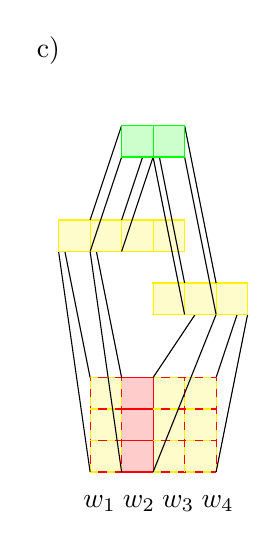
\begin{tikzpicture}[
  hid/.style 2 args={
    rectangle split,
    draw=#2,
    rectangle split parts=#1,
    fill=#2!20,
    outer sep=1mm},
  hidr/.style 2 args={
    rectangle split,
    rectangle split horizontal,
    draw=#2,
    rectangle split parts=#1,
    fill=#2!20,
    outer sep=1mm}
]


  \node [anchor=west] (label) at (-.8, 5.35) {c)};
\fill[red!20!] (0,0) rectangle (1.6,1.2);
\node (w1) at (.12, -.4) {$w_1$};
\node (w1) at (.62, -.4) {$w_2$};
\node (w1) at (1.12, -.4) {$w_3$};
\node (w1) at (1.62, -.4) {$w_4$};

\fill[yellow!20!] (0,0) rectangle (.4,1.2);
\fill[yellow!20!] (.8,0) rectangle (1.6,1.2);
\draw[step=.4cm,red] (0,0) grid (1.6,1.2);
\draw[step=.4cm,yellow, dashed] (0,0) grid (.4,1.2);
\draw[step=.4cm,yellow,dashed] (.8,0) grid (1.6,1.2);

\draw [] (0,1.2) -- (-.4, 3.2);
\draw [] (.4,1.2) -- (0, 3.2);
\draw [] (0,0) -- (-.4, 2.8);
\draw [] (.4,0) -- (0, 2.8);

\draw [] (.8,1.2) -- (1.6, 2.4);
\draw [] (.8,0) -- (1.6, 2);
\draw [] (1.6,1.2) -- (2, 2.4);
\draw [] (1.6,0) -- (2, 2);

\fill[yellow!20!] (.79,1.99) rectangle (2,2.4);
\draw[step=.4cm,yellow] (.79,1.59 + .4) grid (2,2 + .4);
\fill[yellow!20!] (.79 -1.2, 1.59 + 1.2) rectangle (2.4 - 1.2, 2 + 1.2);
\draw[step=.4cm,yellow] (.79 -1.2, 1.59 + 1.2) grid (2.4 - 1.2, 2 + 1.2);



%\draw  (.8,1.2) -- (1.6, 2.4);
%\draw  (.8,0) -- (1.6, 2);
%\draw  (1.6,1.2) -- (2, 2.4);
%\draw  (1.6,0) -- (2, 2);
%
\draw  (-.4 + .4,3.2) -- (.4, 4.4);
\draw  (0 + .4,3.2) -- (.8, 4.4);
\draw  (-.4 + .4,2.8) -- (.4, 4);
\draw  (0 + .4,2.8) -- (.8, 4);


\draw  (1.2,2.4) -- (.8, 4.4);
\draw  (1.6,2.4) -- (1.2, 4.4);
\draw  (1.2,2) -- (.8, 4);
\draw  (1.6,2) -- (1.2, 4);


\fill[green!20!] (.4,4) rectangle (1.2, 4.4);
\draw[step=.4cm,green] (.4,3.99) grid (1.2,4.4);

%?  \foreach \step in {1,...,6} {
%?    \node[hid={3}{red},rotate=-15,shift={(0,-.1 * \step)}] (e\step) at (.40*\step, -1) {};    
%?  }
%?
%?  \foreach \step in {5,...,6} {
%?    \node[hid={3}{yellow},rotate=-15,shift={(0,-.1 * \step)}] (c\step) at (.40*\step, -1) {};    
%?  }
%? 
%?\node[hidr={5}{yellow}] (conv2) at (2.5,.5) {};
%?
%?\draw[yellow] (1.84,-.82) -- (3.1,.69);
%?\draw[yellow] (1.51,-2.05) -- (3.105,.31);
%?\draw[yellow] (2.61,-1.02) -- (3.49,.69);
%?\draw[yellow] (2.28,-2.25) -- (3.495,.31);
%?
%?  \foreach \step in {2,...,2} {
%?    \node[hid={3}{yellow},rotate=-15,shift={(0,-.1 * \step)}] (c\step) at (.40*\step, -1) {};    
%?  }
%? 
%?\node[hidr={6}{yellow}] (conv1) at (0,.5) {};
%?
%?\node[hid={4}{green}] (s3) at (1.25, 2.5) {};
%\path[->] (concat) edge (s2);

\end{tikzpicture}

\end{document}
